\section{From Physical Predictions to Causal Attribution}
\label{sec:narrative-method}

\subsection{Where Physics Enters the Estimator}

The causal bank is the frozen R11 research implementation. Physics determines the candidate response, rather than supplying a penalty to a learned bus-label classifier. Kirchhoff constraints connect each unmeasured source to all available PMUs. With complex bus voltage $V$, the relevant electrical maps include
\begin{equation}
 I_{\rm bus}=Y_{\rm bus}V,\quad I_{{\rm term},r}=Y_{{\rm term},r}V,\quad
 S_i=V_i I_{{\rm bus},i}^{*}.
 \label{eq:narrative-electrical}
\end{equation}
Terminal-current rows retain transformer ratios, charging and orientation. A terminal current is not the bus injection in the power equation. A line hypothesis changes both the network constraints and the resulting terminal observations; a load hypothesis changes the local input and its dynamic propagation.

On a regular index-one DAE chart, differentiating the algebraic constraint gives the local predictor
\begin{align}
 \delta z&=-g_z^{-1}(g_x\delta x+g_u\delta u),\nonumber\\
 \delta\dot x&=(f_x-f_zg_z^{-1}g_x)\delta x
 +(f_u-f_zg_z^{-1}g_u)\delta u.
 \label{eq:narrative-reduction}
\end{align}
The frozen implementation builds transition/observation operators from the full DAE derivatives, with native terminal-current dependence for each topology. Equation~\eqref{eq:narrative-reduction} explains why an input at an unmeasured bus leaves a network-wide signature. It also explains why a local magnitude threshold alone cannot identify the source. Generator inertia, controls and the load law remain those of the frozen plant; no event-specific plant recalibration occurs here.

\subsection{Ask What Could Have Happened in the Last Ten Seconds}

At report time $t$, screening considers candidate onsets in $[t-10\,\mathrm{s},t]$. For each source and family it asks: if this intervention began at $\tau$, what reports should have arrived from $\tau$ to $t$? Prediction starts from the stored no-event state estimate at $\tau$, not a reset to nominal equilibrium. This matters when a new intervention arrives during recovery from the preceding one.

For a candidate history, the comparison is between a physical prediction and the same observed window,
\begin{align}
 r_{h,W}&=y_W-\widehat y_{h,W},\nonumber\\
 L_{h,W}&=\int p(y_W\mid h,a,\mathcal F_{\tau^-})p(a\mid h,\mathcal F_{\tau^-})\,da.
 \label{eq:narrative-evidence}
\end{align}
Conditional state filtering accounts for the retained physical state and colored instrumental noise. Load amplitude is integrated through the inherited truncated-Gaussian calculation; opening a line uses a switched operator. A finite line-screening response proposes a candidate, and the full switched operator confirms it from the estimated initial state. The rolling screen proposes useful histories; it is not additional independent evidence. A selected suffix is replayed with its original state snapshot, while the sequential likelihood scores each report once.

Supplementary Appendix~I gives the scalar precision/mean update and normalizing integral used for a retained load history. It makes the calculation reproducible without presenting standard Gaussian square completion as a new inference theorem.

\begin{figure*}[t]\centering
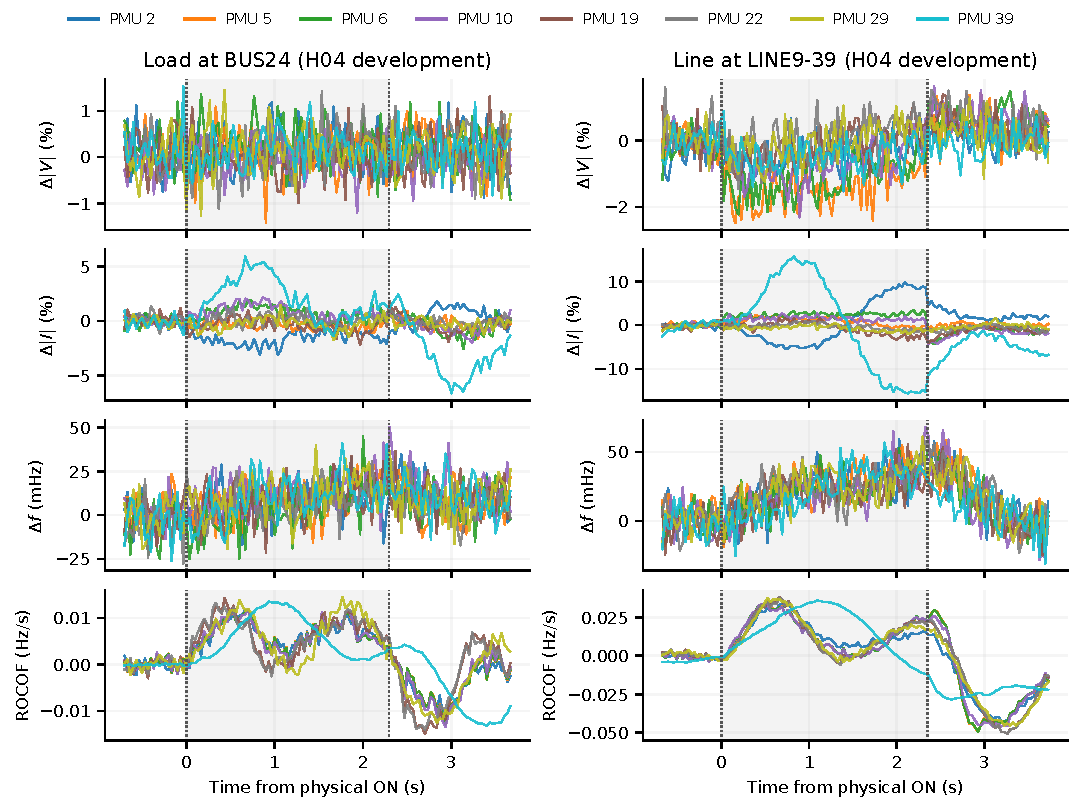
\includegraphics[width=.96\textwidth]{figures/generated/narrative_signals.pdf}
\caption{Why the method compares network responses. Two fixed H04 development examples show the first load and first line intervention in parent H002, measured at all eight PMUs. Shading marks the true intervention interval for retrospective explanation only. The different V/I/frequency/ROCOF responses are observations, not universal family templates: source, operating point and severity also change their shape. Frequency and ROCOF include the frozen causal instrumental estimator.}
\label{fig:narrative-signals}\end{figure*}

\subsection{Keep Reference Error Separate From Event Dynamics}

A wrong observation center can make a quiet network look disturbed. For each fixed network hypothesis $\theta_\ell$, startup estimates
\begin{equation}
 \widehat b_\ell=\overline y_{0:299}-y^{\rm ref}_\ell,
 \qquad b_{\ell,k}=\widehat b_\ell\quad(k\geq300).
 \label{eq:continuous-intercept}
\end{equation}
Angular differences use the common reference consistently. Frequency and ROCOF already have empirical startup centers and receive no extra intercept. The intercept is then frozen: it cannot follow a later load step and erase its signature. This is an observation-discrepancy correction, not recovery of the true impedances or a substitute for an AC-feasible hidden-state estimate. Its uncertainty and the operating-point estimate are treated by substitution.

The preservation mechanism is elementary but useful. For a fixed center, $T_b(y)=y-y^{\rm ref}-b$ satisfies $T_b(y+s)-T_b(y)=s$: a physical response $s$ is not projected away. Updating that center during an intervention would not retain this guarantee. Freezing the center preserves signatures; it does not repair wrong dynamic sensitivities.

Five constant network hypotheses represent nominal, global $\pm2\%$, and selected-branch $\pm3\%$ paired R/X changes. Each propagates its own conditional histories. The outer weight uses a predictive density formed before the current-report state update or screening:
\begin{equation}
 w_{\ell,k}=\frac{w_{\ell,k-1}p_\ell(y_k\mid\mathcal F_{k-1},\widehat b_\ell)}
 {\sum_jw_{j,k-1}p_j(y_k\mid\mathcal F_{k-1},\widehat b_j)}.
 \label{eq:continuous-weights}
\end{equation}
Startup reports are not scored again for network-model selection. Pruning, shared covariance approximations and adaptive history proposals make the result an approximate prequential mixture. We do not claim an optimal Kalman filter, a calibrated event posterior or identification of all line parameters.

\subsection{What $M$ and $\Delta M$ Actually Do}

Let $c$ index an admissible family/source cell. For a bus load the physical index is diagonal, $(i,i,\mathrm{load})$; for a line it is $(i,j,\mathrm{line})$. The implementation stores only the 18 allowed cells. It does not infer every event at every one of the 39 buses.

For network model $\ell$, let $M_{\ell,c,k}$ be the active history mass assigned to cell $c$. The mixed array and its exact increment are
\begin{align}
 M_{c,k}&=\sum_\ell w_{\ell,k}M_{\ell,c,k},\nonumber\\
 \Delta M_{c,k}&=\underbrace{\sum_\ell w_{\ell,k}(M_{\ell,c,k}-M_{\ell,c,k-1})}_{\text{conditional evidence evolution}}\nonumber\\
 &\quad+\underbrace{\sum_\ell(w_{\ell,k}-w_{\ell,k-1})M_{\ell,c,k-1}}_{\text{network-model reweighting}}.
 \label{eq:continuous-delta}
\end{align}
The array is operational: the mixed masses drive decisions. The decomposition identifies whether an attribution changed within the conditional observers or because network hypotheses were reweighted. It is an accounting identity checked by the code, not a new tensor-factorization theorem. A separate cause mass retains the originating intervention after it switches OFF, so the observer can explain recovery without declaring a new event.

The nominal reference runs the same physical/measurement construction with one network hypothesis and its own publication path. Comparing it with the five-model version tests the value and cost of model uncertainty without changing the plant or its source catalog.

\subsection{Emit Decisions Without Resetting the Network}

An alarm, a confirmed family/source diagnosis and an estimated restoration are separate messages. The inherited configuration uses alarm/restoration mass thresholds of 0.99, six confirmation reports for alarm evidence, and 15 reports for restoration confirmation. These numbers are frozen method settings, not calibration guarantees. Additional source/line confirmation and episode-replacement rules remain those of the archived implementation; the configuration is included in the evidence snapshot.

Every emitted message records the latest report used. The observer continues through OFF with its conditional state and covariance; it does not reset to an equilibrium. A later event can begin while the network is still recovering. A source diagnosis emitted after true OFF remains correct eventually but fails the timely-localization metric.

The restricted runtime algorithm is: initialize from the permitted prefix; predict each fixed-model history; score the new report; propose/replay retrospective interventions when supported; mix the history masses; publish a confirmed decision; retain states through restoration. This is model-based Bayesian hypothesis inference. The ExtraTrees comparators are the learned components in this comparison; R11 has no learned bus-label head.
